\section{Understanding and Exploring Data}
\label{section:exploratory_analysis}

Based on \cref{fig:duration_severity,fig:distance_severity}, the MapQuest accidents with severity 4 are much more serious than other severity accidents. These other levels of severity are hard to distinguish from each other. Thus, I decided to focus on severity 4 accidents (from now referred to as "severe") and group the other severity accidents (from now referred to as "non-severe") together.

\subsection{Data Sample Normalization}
In this processed dataset, there are roughly 2.61 million non-severe accidents and only 9000 severe accidents. This discrepancy must be normalized before conducting any further exploratory analysis. I created a Python function to return a random sample of 50000 undersampled non-severe and 50000 oversampled severe accidents.

\subsection{Trends based on Time}
\noindent
Next, I decided to explore if there were trends based on time.

\begin{figure}[H]
    \centering
    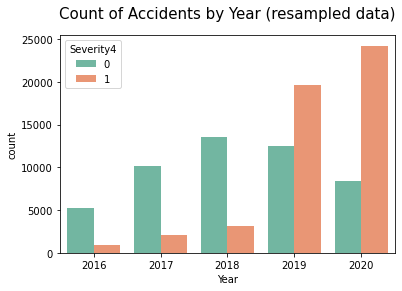
\includegraphics[width=80mm,height=\textheight,keepaspectratio]{images/accident_counts.png}
    \caption{Count of Accidents by Year}
    \label{fig:accidents_year}
\end{figure}

\noindent
Looking at Figure \ref{fig:accidents_year}, it is highly improbable that severe accidents rose by 5 times from 2018 to 2019. To investigate this, I created a heatmap of these severe accidents to see how the data is actually distributed.

\begin{figure}[H]
    \centering
    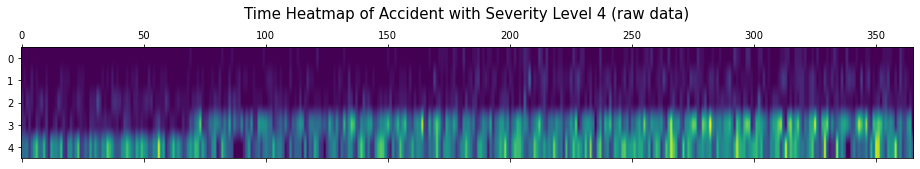
\includegraphics[width=130mm,height=\textheight,keepaspectratio]{images/severe_heatmap.png}
    \caption{Time Heatmap of Severe Accidents}
    \label{fig:severe_heatmap}
\end{figure}

This heatmap strongly indicates that something changed after February 2019, such as the way that MapQuest defines severity or the way they collected data. Since the data after February 2019 is consistent with data in the future, dropping the data before March 2019 is the best choice for analysis and predictions.

\subsection{Log Frequency Normalization}
Next, I decided to analyze the accidents per hour. In \cref{fig:counts_hour}, there are two clear peaks in non-severe accidents occurring at roughly at 7-8 am and 4-5 pm, which likely correlate to maximum traffic times due to work-home commutes.

\begin{figure}[H]
    \centering
    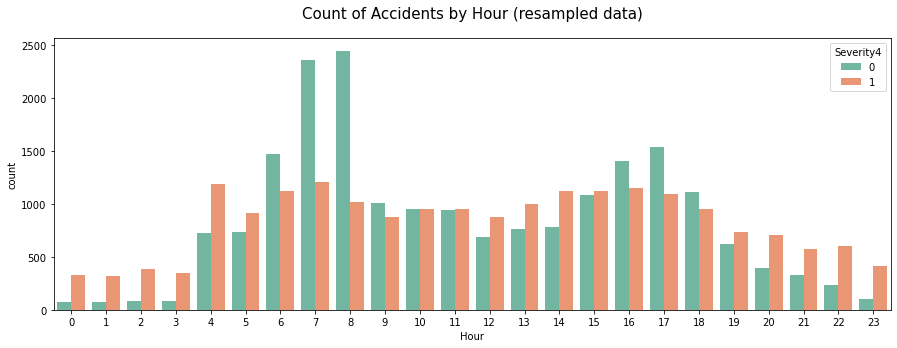
\includegraphics[width=130mm,height=\textheight,keepaspectratio]{images/count_hour.png}
    \caption{Count of Accidents by Hour}
    \label{fig:counts_hour}
\end{figure}

It is also interesting to note that during the hours (early morning or late night) where there were less non-severe accidents, there tended to be relatively greater severe accidents. This observation could be made clearer by using other data for a specific day, hour, or minute. 

Since there are too many classes for a categorical variable for hours, I took the frequency of accidents during the hour. However, since certain hours could have a relatively low frequency, while others could have a relatively high frequency, the log of the frequency is taken to normalize the random continuous variable into a Gaussian distribution. Just in case the frequency is 0, 1 is added to all frequencies before taking the logarithm to prevent undefined values. This log frequency normalization \citep{macurdypencavellog} is defined in Equation \ref{eq:log_freq}.

\begin{equation} \label{eq:log_freq}
    X = \log \left(\left({\frac{n_i}{\sum_{j}^{k}n_j}} \times N_u\right) + 1\right)
\end{equation}

\noindent
where:
\begin{itemize}
    \item $X$ is the resulting continuous random variable after normalization.
    \item $n_i$ is the number of times a possible class of a categorical variable occurs.
    \item $\sum_{j}^{k}n_j$ is the total number of samples.
    \item $N_u$ is the number of unique classes that the categorical variable can take.
\end{itemize}


\begin{table}[H] 
\centering
\begin{tabular}{lll}
Severe & Hour & Hour Freq \\ \hline
1      & 22   & 3         \\
0      & 14   & 2         \\
0      & 5    & 1         \\
0      & 22   & 3         \\
0      & 14   & 2         \\
1      & 22   & 3        
\end{tabular}
\caption{Example Data for Hour Log Frequency Normalization}
\label{table:log_freq}
\end{table}

\noindent
For example, using the example data in Table \ref{table:log_freq}, the hour log frequency normalization for the first row can be performed using Equation \ref{eq:log_freq_example}.

\begin{align} \label{eq:log_freq_example}
    X &= \log \left(\left({\frac{n_i}{\sum_{j}^{k}n_j}} \times N_u\right) + 1\right) \\
    &= \log \left(\left({\frac{3}{6}} \times 24 \right) + 1\right) \\
    &= \log 13 \approx 2.56
\end{align}

\begin{figure}[H]
    \centering
    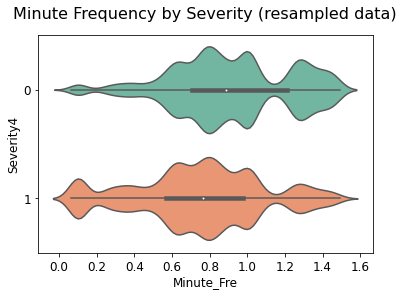
\includegraphics[width=80mm,height=\textheight,keepaspectratio]{images/violin_minute.png}
    \caption{Accidents by Location Frequency}
    \label{fig:violin_minute}
\end{figure}

\subsection{Location}
\cref{fig:violin_lat_lng} shows the distribution of accidents based on latitude and longitude. The violin plots for non-severe and severe accidents seem to be very similar, though there are subtle changes in the ratio of the types of accidents.

\begin{figure}[H]
    \centering
    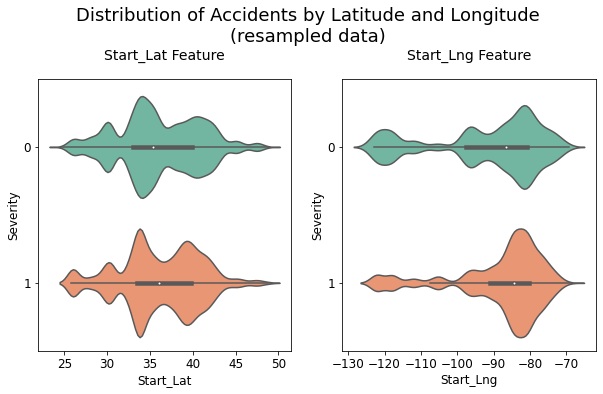
\includegraphics[width=100mm,height=\textheight,keepaspectratio]{images/violin_lat_lng.png}
    \caption{Accidents by Latitude and Longitude}
    \label{fig:violin_lat_lng}
\end{figure}

In \cref{fig:map_accidents}, I plotted the latitude and longitude. I was fascinated to see how clearly the accidents were distributed across the US. The figure clearly shows more densely populated areas tended to have more accidents. More interesting, however, was how the severe accidents seemed to most densely be located in network-like structure. This seemed to indicate the US interstate highway system was where the greatest number of accidents seemed to occur.

\begin{figure}[H]
    \centering
    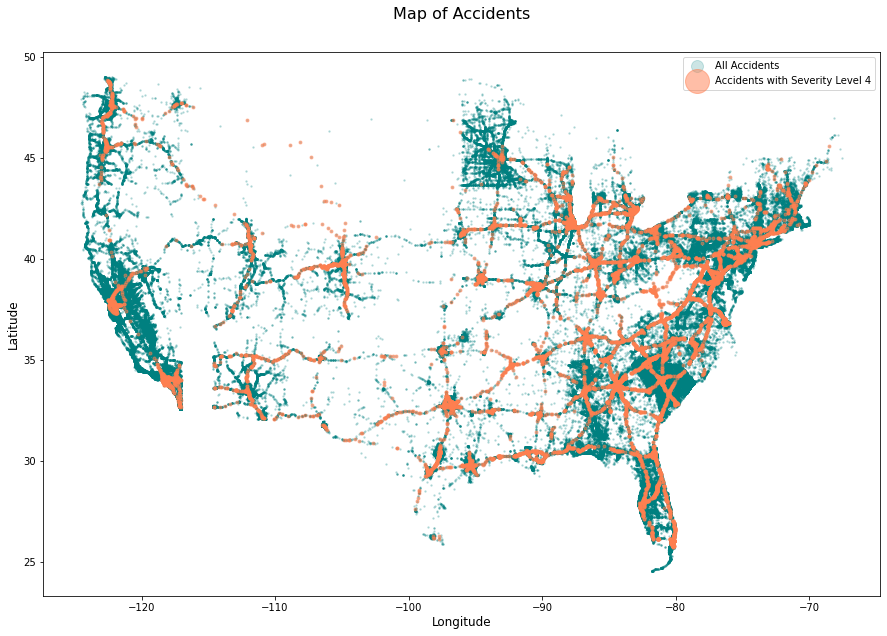
\includegraphics[width=115mm,height=\textheight,keepaspectratio]{images/map_accidents.png}
    \caption{Map of Accidents}
    \label{fig:map_accidents}
\end{figure}

Using Equation \ref{eq:log_freq}, I used the frequency of local indicators such as 'Street', 'City', 'County', 'Zipcode', 'Airport Code', and 'State' to try to capture the clear correlation to the highway accidents in continuous random variables.

\begin{figure}[H]
    \centering
    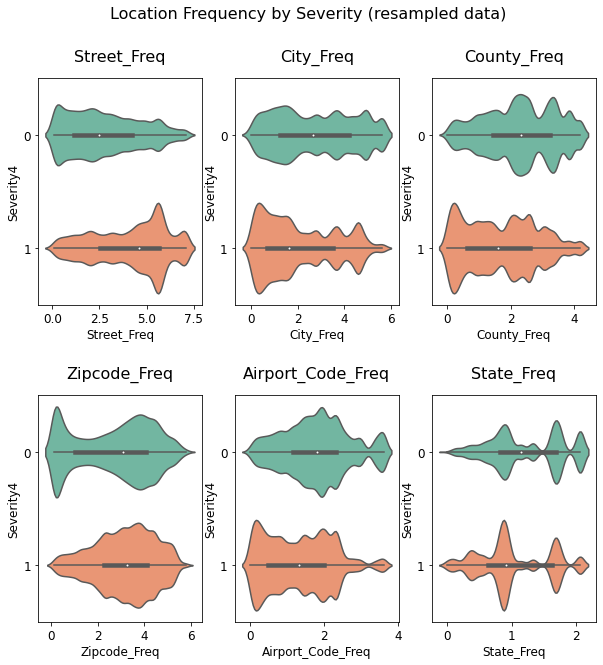
\includegraphics[width=100mm,height=\textheight,keepaspectratio]{images/violin_loc.png}
    \caption{Accidents by Location Frequency}
    \label{fig:violin_loc}
\end{figure}

\subsection{Weather Features}
Since the weather features such as 'Pressure', 'Visibility', and 'Wind Speed' are highly skewed, they must be normalized prior to analysis. A Box Cox transformation \citep{osborne2010improving} can turn non-normal dependent variables into a normal Gaussian shape. By precisely controlling the parameter \(\lambda\), I was able to normalize the weather features.

\begin{equation} \label{eq:boxcox_transform}
    y(\lambda)=
    \begin{cases}
        \frac{y^\lambda - 1}{\lambda} & \lambda \neq 0 \\
        \log{y} & \lambda = 0
    \end{cases}
\end{equation}

Overall, \cref{fig:bar_weather} shows that accidents are little more likely to be serious during rain or snow while less likely on a cloudy day.

\begin{figure}[H]
    \centering
    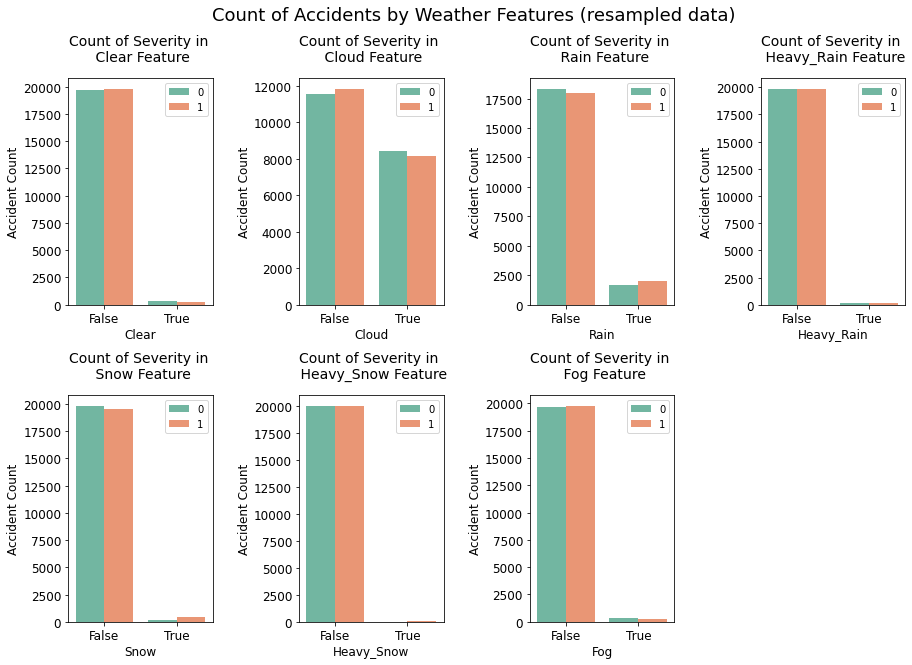
\includegraphics[width=100mm,height=\textheight,keepaspectratio]{images/bar_weather.png}
    \caption{Accidents by Weather}
    \label{fig:bar_weather}
\end{figure}

\section{Point of Interest Features}
\noindent
\cref{fig:accidents_poi} shows the number of accidents that occurred at Points of Interest (POI).

\begin{figure}[H]
    \centering
    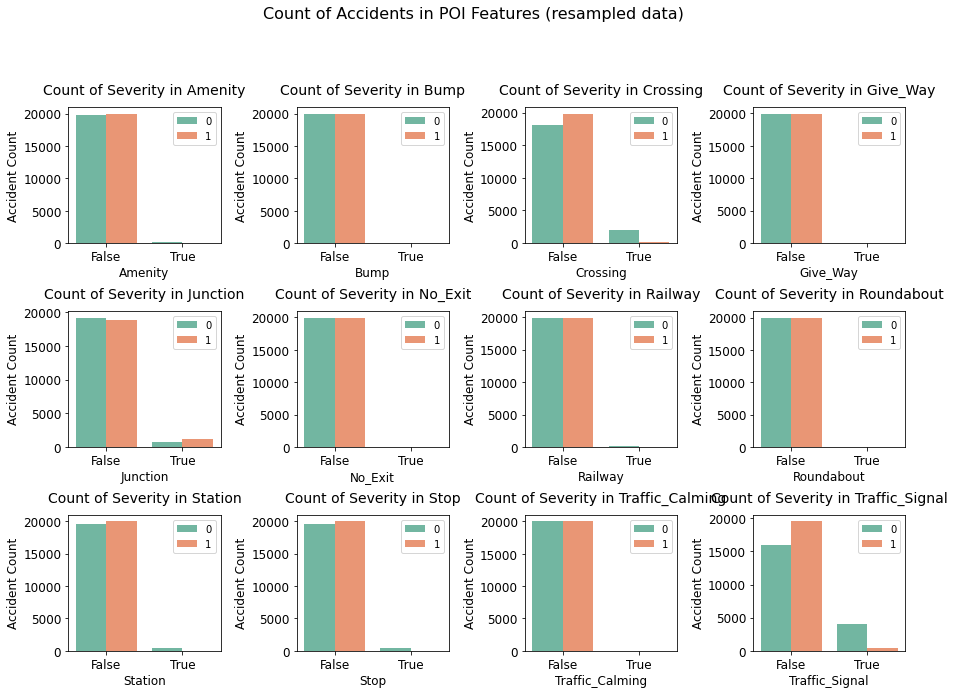
\includegraphics[width=130mm,height=\textheight,keepaspectratio]{images/accidents_poi.png}
    \caption{Accidents by Location Frequency}
    \label{fig:accidents_poi}
\end{figure}

Accidents near traffic signal and crossing are much less likely to be serious accidents while little more likely to be serious if they are near the junction. This may occur because drivers usually slow down in front of crossing and traffic signal but junction and severity are highly related to speed. The other POI features have such little severe accidents that it is hard to tell their relation with severity from plots.

\subsection{Heatmap Correlation}
After all the normalization and processing performed, the following correlation heatmap was derived.

\begin{figure}[H]
    \centering
    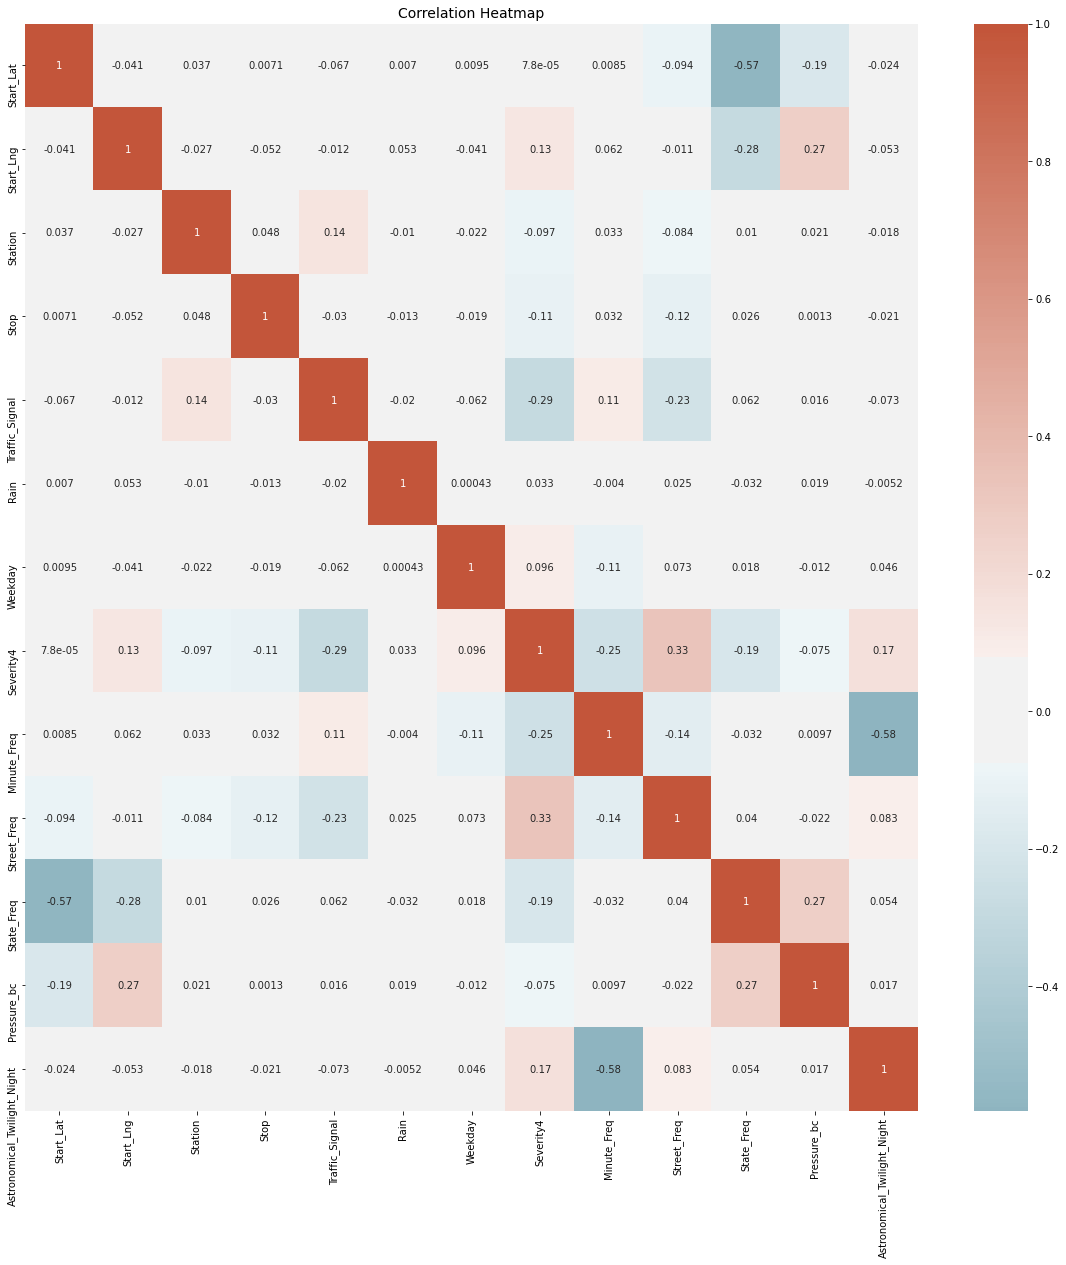
\includegraphics[width=80mm,height=\textheight,keepaspectratio]{images/corr_heatmap.png}
    \caption{Correlation Heatmap}
    \label{fig:corr_heatmap}
\end{figure}

\noindent
This heatmap represents the Pearson correlation coefficient (Equation \ref{eq:correlation_coefficient}) for each pair of continuous random variables in the dataset.

\begin{equation} \label{eq:correlation_coefficient}
    r = \frac{N\sum{XY}-(\sum{X}\sum{Y})}{\sqrt{ [N \sum{x^2}-(\sum{x})^2 ][N \sum{y^2}-(\sum{y})^2 }]}
\end{equation}

The Correlation Heatmap is promising as it shows both mildly strong positive and negative correlations of the various data columns to the severity, while being minimally correlated to each other. 

This should in theory should enable enable a predictive model to optimize weights of select factors in order to derive a strong fit.